\documentclass[12pt , letterpaper]{article}
\title{InlineMathMode (Trignometry)}
\author{Avinash Nair}
\usepackage{graphicx}
\graphicspath{{figures/}}

\begin{document}
\maketitle
This will be overview of Trignometry.
\newline By Pythagoreas Theorem, we know that
$$a^2 + b^2 =c^2$$
\begin{figure}[h]
    \centering
    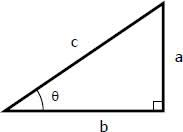
\includegraphics[width=0.50\textwidth]{fig1}
\end{figure}
Where, \emph{a} and \emph{b} are shorter sides of right angled triangle
and \emph{c} is the hyptenuse.
we define,
\begin{equation}
    \sin(\theta) = \frac{a}{c}
\end{equation}
\begin{equation}
    \cos(\theta) = \frac{b}{c}
\end{equation}
\begin{equation}
      \tan(\theta) = \frac{a}{b}
\end{equation}
\end{document}